\newpage
\section{Ideal Simulations}
\subsection{Simulation Results}
Below in the Figure \ref{simulation}, the simulation model schematic can be seen.

\begin{center}
\begin{figure}[H]
\centering
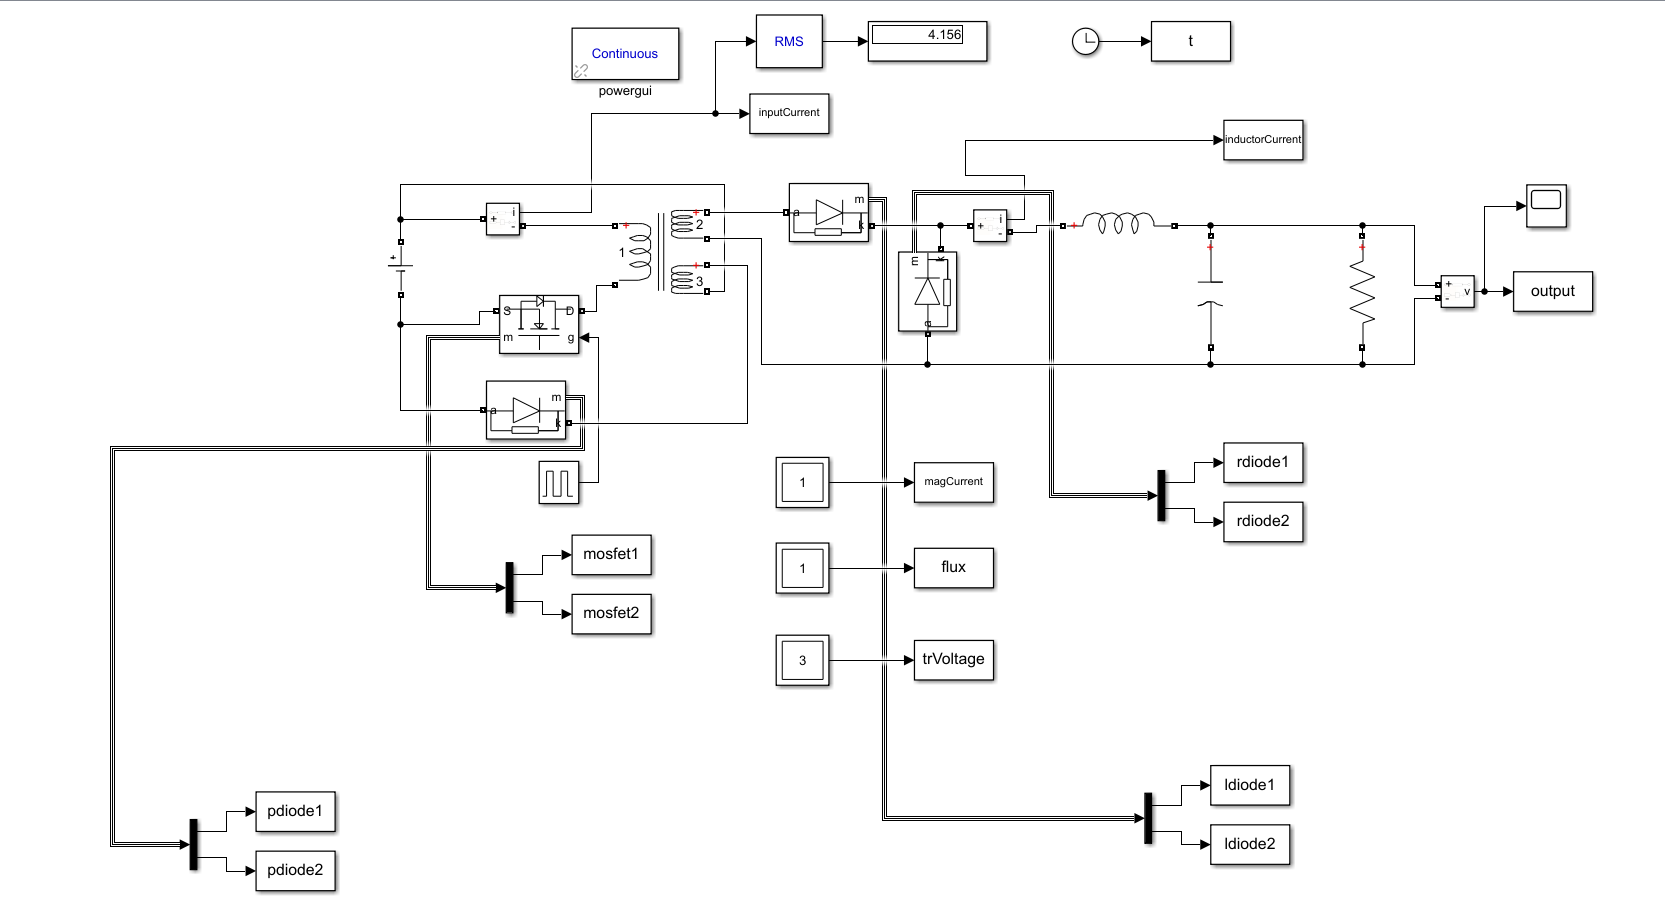
\includegraphics [width=15 cm]{simulation.png}
\caption{Simulation model}
\label{simulation}
\end{figure}
\end{center}

First, we simulated the ideal models in order to see the overall system operation. It is open-loop operation simulation and we would like to validate the duty cycles, operation principle and validity of our selections.

\begin{center}
\begin{figure}[H]
\centering
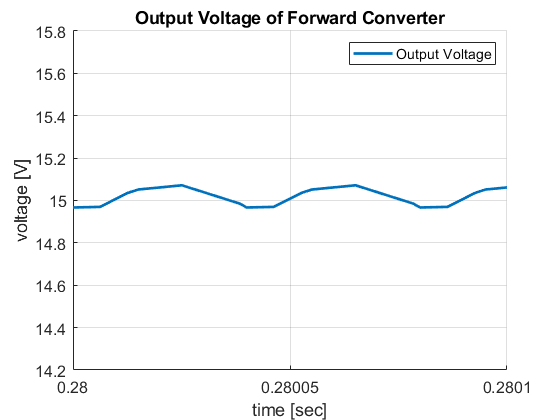
\includegraphics [width=12 cm, height= 8 cm]{output_voltage.png}
\caption{Output waveform of the forward converter under 48V operation}
\label{Output48}
\end{figure}
\end{center}

\begin{figure}[H]
\centering
\begin{subfigure}{7 cm}
  \centering
  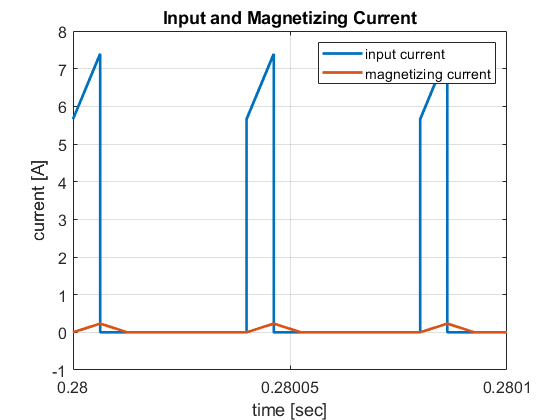
\includegraphics[width=7 cm]{input_current}
  \caption{Input and Magnetizing Current}
  \label{fig:input_current_48}
\end{subfigure}%
\begin{subfigure}{7 cm}
  \centering
  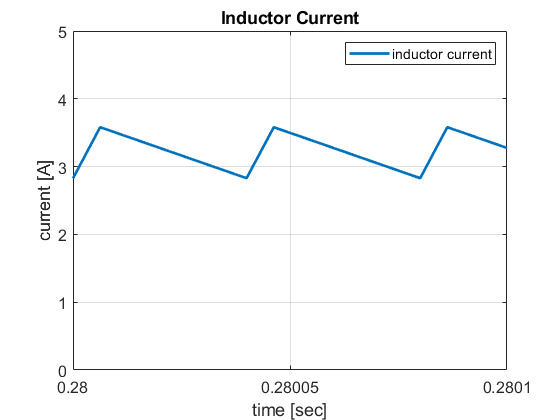
\includegraphics[width=7 cm]{inductor_current}
  \caption{Inductor Current}
  \label{fig:inductor_current_48}
\end{subfigure}
\caption{Forward converter input and inductor current under 48V input operation}
\label{fig:current_48}
\end{figure}


\begin{center}
\begin{figure}[H]
\centering
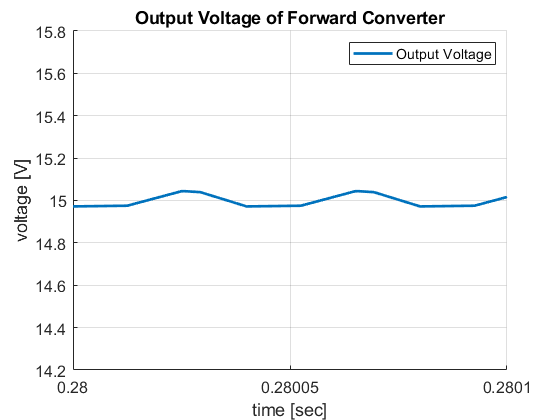
\includegraphics [width=12 cm, height= 8 cm]{output_voltage_24.png}
\caption{Output waveform of the forward converter under 24V operation}
\label{Output24}
\end{figure}
\end{center}

\begin{figure}[H]
\centering
\begin{subfigure}{7 cm}
  \centering
  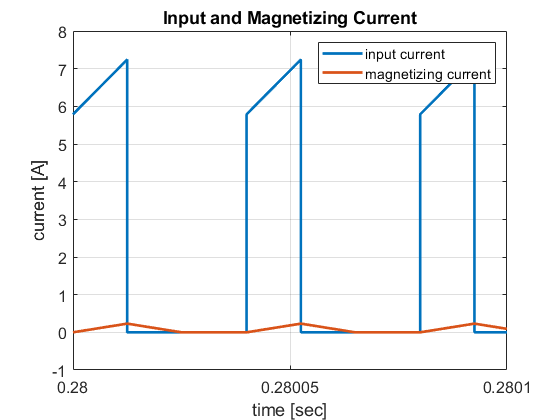
\includegraphics[width=7 cm]{input_current_24}
  \caption{Input and Magnetizing Current}
  \label{fig:input_current_24}
\end{subfigure}%
\begin{subfigure}{7 cm}
  \centering
  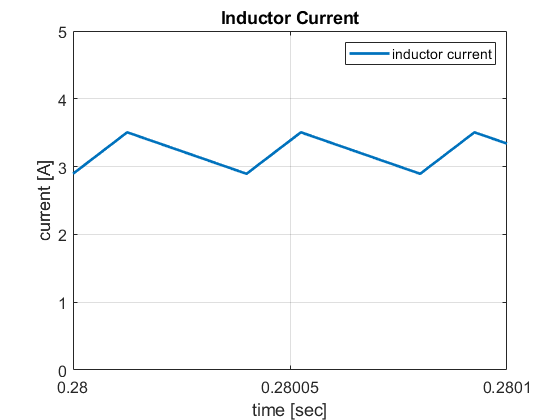
\includegraphics[width=7 cm]{inductor_current_24}
  \caption{Inductor Current}
  \label{fig:inductor_current_24}
\end{subfigure}
\caption{Forward converter input and inductor current under 24V input operation}
\label{fig:current_24}
\end{figure}


As we can see from the Fig. \ref{Output24} and \ref{Output48} the output ripple is below $2\%$. The operation is stable and the duty cycles are as expected. However, when non-idealities are presented the duty cycle values will be re-calculated in order to compansate the voltage drops of losses and diodes etc. 

Also, from the Fig. \ref{fig:current_24} and \ref{fig:current_48}, we can observe the magnetizing current is as expected around $0.3A$ and the inductor ripple is around $0.6A$ for both operations. These results show that our calculations are valid. Now we are going to add non-idealities of the circuit.







